
%%% Preamble
\documentclass[paper=a4, fontsize=11pt]{scrartcl}
\usepackage[T1]{fontenc}
\usepackage{fourier}
\usepackage{listings}
\usepackage[english]{babel}															% English language/hyphenation
\usepackage[protrusion=true,expansion=true]{microtype}	
\usepackage{amsmath,amsfonts,amsthm} % Math packages
\usepackage[pdftex]{graphicx}	
\usepackage{url}
\usepackage{color}


%%% Custom sectioning
\usepackage{sectsty}
\allsectionsfont{\centering \normalfont\scshape}


%%% Custom headers/footers (fancyhdr package)
\usepackage{fancyhdr}
\usepackage{listings}
\pagestyle{fancyplain}
\fancyhead{}											% No page header
\fancyfoot[L]{}											% Empty 
\fancyfoot[C]{}											% Empty
\fancyfoot[R]{\thepage}									% Pagenumbering
\renewcommand{\headrulewidth}{0pt}			% Remove header underlines
\renewcommand{\footrulewidth}{0pt}				% Remove footer underlines
\setlength{\headheight}{13.6pt}


%%% Equation and float numbering
\numberwithin{equation}{section}		% Equationnumbering: section.eq#
\numberwithin{figure}{section}			% Figurenumbering: section.fig#
\numberwithin{table}{section}				% Tablenumbering: section.tab#


%%% Maketitle metadata
\newcommand{\horrule}[1]{\rule{\linewidth}{#1}} 	% Horizontal rule

\title{
	%\vspace{-1in} 	
	\usefont{OT1}{bch}{b}{n}
	\horrule{0.5pt} \\[0.4cm]
	\huge CS150A Homework 3 -- Writing \\
	\horrule{2pt} \\[0.5cm]
}
\author{
	\normalfont 								\normalsize
	School of Information Science and Technology \\
	[-3pt]		\normalsize
	\today
}
\date{}
\begin{document}
\maketitle
\section{Concurrency Control(20 pts)}

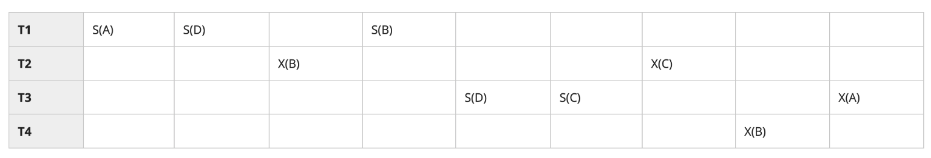
\includegraphics[height=2.5cm]{deadlock.png}
\begin{itemize}
        \item [1.] Draw the "waits-for" graph and explain whether or not there is a deadlock. \\~\\~\\~\\~\\
\item [2.] If we try to avoid deadlock by using the wait-die deadlock avoidance policy, would any transactions be aborted? Assume T1 $<$ T2 $<$ T3 $<$ T4 for the priority.\\~\\~\\~\\
\end{itemize}

\section{Recovery(30 pts)}
% 	Consider the following relations with underlined primary keys:\\
% 	\indent\indent Student (sname, \underline{sid}, gpa, level, deptid)\\
% 	\indent\indent Dept (dname, \underline{deptid})\\
%     \indent\indent Course (\underline{cid}, cname, deptid, units)\\
%     \indent\indent Takes (\underline{sid}, \underline{cid})\\
The database has just crashed owing to the operator error, and this time you follow the recovery process with the \textbf{STEAL/NO FORCE} policy. You boot the database server back up, and find logging information on disk at the following tables:\\

\begin{minipage}{\textwidth}
\begin{minipage}[t]{0.6\textwidth}

\makeatletter\def\@captype{table}
\centering
    \begin{tabular}{|c|c|c|}
    \hline
        \textbf{LSN} & \textbf{Record} & \textbf{prevLSN} \\ \hline
        30 & update: T3 writes P5 & null \\ \hline
        40 & update: T4 writes P1 & null \\ \hline
        50 & update: T4 writes P5 & 40 \\ \hline
        60 & update: T2 writes P5 & null \\ \hline
        70 & update: T1 writes P2 & null \\ \hline
        80 & Begin Checkpoint & - \\ \hline
        90 & update: T1 writes P3 & 70 \\ \hline
        100 & End Checkpoint  & - \\ \hline
        110 & update: T2 writes P3 & 60 \\ \hline
        120 & T2 commit & 110 \\ \hline
        130 & update: T4 writes P1 & 50 \\ \hline
        140 & T2 end & 120 \\ \hline
        150 & T4 abort & 130 \\ \hline
        160 & update: T5 writes P2 & null \\ \hline
        180 & CLR: undo T4 LSN 130 & 150 \\ \hline
    \end{tabular}
    \caption{log records}
\label{record}
\end{minipage}
\begin{minipage}[t]{0.48\textwidth}
\makeatletter\def\@captype{table}
\centering
\begin{tabular}{|c|c|c|}
\hline
    \textbf{Transaction ID} & \textbf{LastLSN} & \textbf{Status} \\ \hline
    T1 & 70 & Running \\ \hline
    T2 & 60 & Running \\ \hline
    T3 & 30 & Running \\ \hline
    T4 & 50 & Running \\ \hline
\end{tabular}
\caption{Transaction Table}
\\~\\
\label{sample-1}
\begin{tabular}{|c|c|}
\hline
    \textbf{Page ID} & \textbf{RecLSN} \\ \hline
    P5 & 50 \\ \hline
    P1 & 40 \\ \hline
    ~ & ~ \\ \hline
    ~ & ~ \\ \hline
\end{tabular}
\caption{Dirty Page Table}
\label{sample-2}
\end{minipage}
\end{minipage}

\begin{enumerate}
    \item Was the update to page 5 at LSN 60 successfully written to disk? Also, was the update to page 2 at LSN 70 successfully written to disk? Please explain both cases briefly.\\
    \\
    \\
    \\
    \\
    \\
    \item At the end of the Analysis phase, what transactions will be in the transaction table, and with what lastLSN and Status values? What pages will be in the dirty page table, and with what recLSN values?
\begin{table}[h]
\centering
    \begin{subtable}
    \begin{tabular}{|c|c|c|}
    \hline
    \textbf{Transaction ID} & \textbf{LastLSN} & \textbf{Status} \\ \hline
    & & \\ \hline
    & & \\ \hline
    & & \\ \hline
    & & \\ \hline
    \end{tabular}
    \label{sample-1}
    \end{subtable}
    \qquad
    \begin{subtable}
    \begin{tabular}{|c|c|}
    \hline
    \textbf{Page ID} & \textbf{RecLSN} \\ \hline
     &  \\ \hline
     &  \\ \hline
    ~ & ~ \\ \hline
    ~ & ~ \\ \hline
    \end{tabular}      
    \label{tab:secondtable}
    \end{subtable}
\end{table}
\item At which LSN in the log should redo begin? Which log records will be redone (list their LSNs)? All other log
records will be skipped.

\end{enumerate}


\section{Parallel Query Processing(15 pts)}

We've discussed 4 kinds of parallel join in class:
\begin{itemize}
    \item \textbf{Parallel Hash Joins}: Use hash partitioning on both relations with the same hash function, then perform a normal hash join on each machine independently.
    \item \textbf{Parallel Sort Merge Join}: Use range partitioning with the same ranges on both relations, then perform sort merge join on each machine independently.
    \item \textbf{One-sided shuffle Join}: When one relation's data is already partitioned the way we want (hash partitioned or range partitioned on a key), just partition the other relation, then run local join (using any algorithm) at every node and union results.
    \item \textbf{Broadcast Join}: If one relation is small, send it to all nodes that have a partition of the other relation. Do a local join at each node (using any algorithm) and union results.
\end{itemize}

\par In shared nothing, the machines communicate with each other solely through the network by sending data to each other. Here, network cost is referred to the amount of data sent between machines. 
\par Now we have a Relation R that has 10,000 pages, round-robin partitioned across 4 machines (M1, M2, M3, M4). Relation S has 20 pages, all of which are only stored on M1. We want to join R and S on the condition R.col = C.col. Assume the size of each page is 1 KB. 

\begin{enumerate}
    \item Which type of join would have the lowest network cost in this scenario?
    \begin{enumerate}
        \item Parallel Hash Joins
        \item Parallel Sort Merge Join
        \item One-sided shuffle Join
        \item Broadcast Join
    \end{enumerate}

    \item How many KB of data must be sent over the network to join R and S using this join method? \\ \\ \\

    \item Would the amount of data sent over the network change if R was hash or range partitioned among the 4 machines rather than round-robin partitioned using this join method? 
    \begin{enumerate}
        \item The network cost will not change under both of the partitioning methods.
        \item The network cost will change under both of the partitioning methods.
        \item The network cost will only change under range partitioning.
        \item The network cost will only change under hash partitioning.
    \end{enumerate}

\end{enumerate}
\\~\\





\section{Distributed Transaction(15 pts)}
\begin{itemize}
\item [1.] Suppose we have one coordinator and four participants. It takes 40ms for a coordinator to send messages to all participants; 5,10,20 and 25ms for participant 1,2,3 and 4 to send a message to the coordinator respectively; and 15 ms for each machine to generate and flush a record. Assume for the same message, each participant receives it from the coordinator at the same time. \\
    Under proper 2PC and logging protocols, how long does the whole 2PC process (from the beginning to the coordinator's final log flush) take for a successful commit in the best case?(Please write down your analysis for the question.)\\~\\~\\~\\~\\
\end{itemize}

\section{No SQL(20 pts)}
 Answer the questions about scaling, you need to give a brief analysis.
\begin{itemize}
\item [1.] A small startup realizes that its current database can’t sustain their growing workloads. Given
that these workloads involve lot of write but few reads, should it invest in more partitioning or
more replication?\\~\\~\\~\\~\\~\\
\item [2.] A mechanical failure causes some of the startup’s database machines to permanently crash,
losing data in the process. If the startup wants to prevent similar losses in the future, should it
invest more in partitioning or more replication?
\end{itemize}

\end{document}